\chapter{Experimentelle Untersuchungen}
\chaptermark{Exp. Untersuchungen}

Um die Wirksamkeit der Parallelisierung der N++-Bibliothek in C++ zu bewerten, wird ein umfassender Benchmark-Test durchgeführt. Dieser Test umfasst verschiedene Kombinationen von Threads, Anzahl an Datensätzen und verschiedenen Computern mit verschiedenen Prozessorarchitekturen, um die Auswirkungen der Implementierung auf die Leistung der Bibliothek unter unterschiedlichen Bedingungen zu untersuchen.

\section{Testumgebung}

Das C++ Programm wurde unter Einbindung der N++-Bibliothek auf dem jeweiligen System selbst kompiliert. Dabei wurde die Optimierungsstufe O2 verwendet, welche eine für Produktionssoftware gängige Optimierungsstufe ist. Die O2 Optimierungsstufe wendet fast jede Compileroptimierung an, die die Compiler zu bieten haben. Dabei werden lediglich als sehr unsicher eingestufte Optimierungen ausgelassen. Auf Linux wurde der GCC Compiler (Version 12.2.0-14) und auf MacOS der Clang Compiler (Version 1500.3.9.4) verwendet, um native Binärdateien für die spezifische Prozessorarchitektur zu kompilieren. Das heißt, das Programm wurde nicht unter Emulation sondern vollständig nativ ausgeführt.

Die Tests wird mit unterschiedlichen Thread-Anzahlen ausgeführt, darunter 10, 8, 6, 4 und 2 gleichzeitig laufenden Threads, um den Einfluss der Parallelisierung auf die Ausführungsgeschwindigkeit zu untersuchen. Zusätzlich wird das Programm auch mit einem einzelnen Thread ausgeführt, um einen Vergleich mit der vorausgegangenen Implementierung herstellen zu können. Für jede Thread-Anzahl werden außerdem verschiedene Größen an Datensätzen getestet. Die Größe der Datensätze wird über die Anzahl an Partitionen spezifiziert. Eine Partition bedeutet dabei, dass die gesamte Datenmenge verwendet wird, wohingegen 4 Partitionen bedeuten, dass nur ein Viertel, also 25\% der Datenmenge verwendet werden. Das Programm wird in diesem Test mit 1, 2, 4 und 8 Partitionen getestet, wobei es auf dem langsamsten Computer nur auf 4 und 8 beschränkt wurde.

Für jede Kombination von Threads und Partitionen werden mindestens 5 Testläufe durchgeführt, um robuste Durchschnittswerte zu erhalten und Schwankungen zu minimieren. Gemessen wird die benötigte Zeit für den gesamten Programmdurchlauf in Sekunden. Vor jedem Durchlauf werden die Testgeräte auf einen neutralen Zustand zurückgesetzt, um faire Vergleichsbedingungen sicherzustellen. Dies wird gewährleistet, indem gleiche Seeds für die Zufallszahlgeneratoren verwendet werden, und sichergestellt wird, dass keine anderen Programme laufen.
Das Ergebnis jedes Programmdurchlaufs wird in eine Datei geschrieben, um vergleichen zu können, ob mit verschiedenen Anzahlen von Threads die gleichen Ergebnisse berechnet werden.

Nach Abschluss der Testläufe werden die erzielten Ergebnisse automatisch analysiert und Durchschnittswerte für jede Kombination von Threads und Partitionen berechnet. Diese Durchschnittswerte dienen dazu, die möglichen Schwankungen der Testabläufe auszugleichen, und ein neutraleres Ergebnis zu liefern.

\section{Getestete Hardware}
\sectionmark{Hardware}

Als erstes Testsysten kommt ein MacBook Pro 16 Zoll Laptop mit dem M1 Pro Prozessor, der im MacBook Pro 16 Zoll verwendet wird zum Einsatz. Der M1 Pro wurde 2021 vorgestellt und ist eine hochskalierte Version des M1 Prozessors. Er verfügt über insgesamt 12 CPU-Kerne, darunter 8 Hochleistungs- und 4 Effizienzkerne \citep{MacBook_Technische_Daten}. Die Hochleistungskerne sind für rechenintensive Aufgaben konzipiert, während die Effizienzkerne für weniger anspruchsvolle Aufgaben und eine Reduzierung des Energieverbrauchs optimiert sind.
In Bezug auf die Leistung bietet der M1 Pro Prozessor eine sehr beeindruckende Single-Core-Leistung und ist das performanteste der getesteten Systeme. Die Hauptspeichergröße beträgt 16 GB, welche mit einer Speicherbandbreite von 200 GBit/s \citep{MacBook_Technische_Daten} angebunden sind. Auch die Cache-Größe des Prozessors ist sehr hoch, was die Latenz bei Speicherzugriffen zusätzlich vermindern kann.
Verwendet wurde MacOS Sonoma 14.5 mit dem Darwin Kernel Version 23.5.0 und Clang Version 1500.3.9.4.

Als Desktopprozessor wurde der AMD Ryzen 5 3600XT getestet, welcher ein Prozessor aus der Ryzen 3000-Serie von AMD ist, der im Jahr 2020 eingeführt wurde. Er verfügt über insgesamt 6 CPU-Kerne und 12 Threads auf Basis der Zen 2-Architektur, welche auch im Servermarkt verbreitet ist. Es handelt sich um einen Desktopprozessor mit einer maximalen Leistungsaufnahme von 95 Watt \citep{Ryzen_Technische_Daten}.
Der Prozessor unterstützt DDR4-RAM mit unübertakteten Geschwindigkeiten von bis zu 3200 MHz \citep{Ryzen_Technische_Daten}. Die genaue Speicherbandbreite und Größe hängt von der verwendeten RAM-Konfiguration ab, da Desktop Prozessoren modular in verschiedene Systeme eingebaut werden können.
In Bezug auf den Cache verfügt der Ryzen 5 3600XT über 32KB L1-Cache, 512KB L2-Cache und 32MB L3-Cache \citep{Ryzen_Technische_Daten}. In der Konfiguration des Testcomputers sind 16GB DDR4 Speicher mit 3600 MHz verbaut, und der Prozessor wird mit einer Wasserkühlung gekühlt, was für eine gleichmäßige und robuste Kühlung sorgt. Als Betriebssystem kam Fedora 40 mit dem Linux Kernel der Version 6.8 zum Einsatz.

Um auch ein System mit begrenzter Leistung zu testen wurde die Implementierung auch auf einem  Raspberry Pi 3 getestet, welcher ein Single-Board-Computer ist, der von der Raspberry Pi Foundation entwickelt wurde. Ein Single-Board-Computer ist eine vollständige Computerplatine, die alle erforderlichen Komponenten wie Prozessor, Speicher, Ein- und Ausgabeanschlüsse und Stromversorgung auf einer einzigen Platine vereint. Der Raspberry Pi 3 wurde 2016 veröffentlicht und basiert auf einem ARM Cortex-A53 Quad-Core-Prozessor mit einer Taktfrequenz von 1,2 GHz und 1 GB LPDDR2-RAM \citep{RaspberryPi_Technische_Daten}.
Der Raspberry Pi 3 ist aufgrund seiner geringen Größe, seines geringen Stromverbrauchs und seiner vielfältigen Einsatzmöglichkeiten beliebt. Er wird häufig in Bildungsprojekten, Hobbyprojekten, Heimautomatisierungssystemen und als kostengünstige Entwicklungsumgebung für Softwareentwickler eingesetzt. Trotz seiner begrenzten Leistungsfähigkeit erfüllt der Raspberry Pi 3 wichtige Funktionen in verschiedenen Anwendungsbereichen aufgrund seiner Kompaktheit und seines erschwinglichen Preises.
Aufgrund der begrenzten Leistung und der damit verbundenen Laufzeiten konnte der Testablauf nicht vollständig durchgeführt werden. Es wurden maximal 4 Threads getestet, und die Partitionen wurden auf 8 und 4 begrenzt. Die Linux Kernel Version 6.6 kam auf Raspberry Pi OS Lite 12 in der 64-Bit Version zum Einsatz.

Um die Skalierbarkeit und das Verhalten der Algorithmen in unterschiedlichsten Umgebungen zu beleuchten, wurden die Benchmarks zusätzlich auf einem VPS-Server des Anbieters Contabo durchgeführt. Diese Wahl bot gleich zweifache Vorteile: Zum einen ermöglichte sie die Evaluierung der Algorithmenleistung in einer Cloud-Umgebung, die in der heutigen Anwendungslandschaft immer relevanter wird, zum anderen bietet sie einen modernen performanten Prozessor, welche jedoch aufgrund der Virtualisierung auf 2 Kerne beschränkt ist.
Der Server verfügt über einen AMD EPYC 7282 Prozessor, der speziell für rechenintensive Aufgaben in Serverumgebungen entwickelt wurde. Mit seinen 16 Kernen und 32 Threads bietet er eine beachtliche Rechenleistung. Der Basistakt liegt bei 2,8 GHz und der Cache ist 64 MB groß \citep{Epyc_Specifications}.
Von diesem leistungsstarken Prozessor stehen dem VPS-Server lediglich 2 Kerne und 4 GB Arbeitsspeicher zur Verfügung. Diese Einschränkung sollte Aufschluss darüber geben, wie effizient die Algorithmen mit limitierten Ressourcen umgehen können und wie sie in skalierbaren Umgebungen performen. Der verwendete Linux-Kernel war die Version 6.1.0-21 auf Debian 12.

\section{Benchmark Script}

Aus 6 verschiedenen Anzahlen an Threads, 4 verschiedenen Größen der Datensätze und 5 Durchläufen pro Kombination ergeben sich 120 einzelne Tests, die pro System ausgeführt werden müssen.
Um diese Arbeit zu erleichtern und einen reproduzierbaren Testprozess zu ermöglichen wurde ein Skript geschrieben, welches alle Tests nacheinander automatisch ausführt.

Das Skript misst die benötigten Laufzeiten der Durchläufe und schreibt nach jedem Durchlauf die benötigte Zeit in eine Datei. Zusätzlich werden die Zeit und Informationen zu jedem Durchlauf auch in eine CSV-Datei geschrieben, um das Auswerten der Benchmarks auf einem System durch nur eine einzige Datei zu ermöglichen.

Als Parameter ist es möglich, die maximale Anzahl an Threads festzulegen. So ist es beispielsweise auf einem Raspberry Pi sinnvoll, das Programm nur mit maximal 4 Threads zu testen, da er nur über 4 Kerne verfügt.

Das Skript ist simpel und wurde in Bash geschrieben, was die Portabilität zwischen Linux und MacOS gewährleistet. Dabei wurde jedoch das Programm bc verwendet, welches auf den meisten Linux-Distributionen standardmäßig nicht vorinstalliert ist.

\begin{figure}[H]
\begin{minted}
[
frame=lines,
framesep=2mm,
baselinestretch=1.2,
fontsize=\footnotesize,
linenos
]{bash}
#!/bin/bash
ATTEMPTS=5
PARTITIONS=(8 4 2 1) # Verschiedene Partitionen zum Testen
THREADS=(10 8 6 4 2 1) # Verschiedene Thread Anzahlen zum Testen
AVAILABLE_THREADS=10 # Maximal verfügbare Anzahl an Threads für aktuelles System

function run_attempt {
    # Hier wird ein Durchlauf durchgeführt und getestet
}

# Test für jede mögliche Kombination durchführen
for partition in ${PARTITIONS[@]};do
  for threads in ${THREADS[@]};do
      if ((threads <= AVAILABLE_THREADS));then
        for ((i = 1; i <= ATTEMPTS; i++)); do
          run_attempt "$threads" "$partition" "$i"
        done
      fi
    done
done
\end{minted}
\caption{Vereinfacht dargestelltes Benchmark Skript. Es testet die benötigte Laufzeit der Implementierung mit verschiedenen Thread-Anzahlen und Datensatzgrößen.}
\label{fig:benchmark_script_code}
\end{figure}

\section{Ergebnisse}

\begin{figure}[H]
\centering
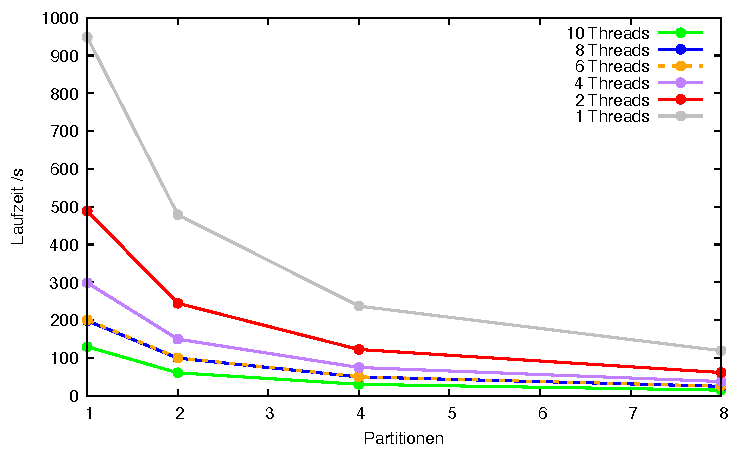
\includegraphics[width=0.8\textwidth]{../results/plots/m1pro/comp_all_threads.pdf}
\caption{Leistungstest auf Apple M1 Pro: Einfluss von Thread-Anzahlen auf Verarbeitungszeit bei variierenden Datensatzgrößen}
\label{fig:m1pro_benchmark_threads}
\end{figure}

Die Analyse der Benchmark-Ergebnisse auf dem M1 Pro-Prozessor aus Abbildung \ref{fig:m1pro_benchmark_threads} liefert wertvolle Einblicke in die Effektivität von Parallelisierung des Programms. Durch Tests mit 10, 8, 6, 4, 2 und 1 Threads konnte eine größtenteils lineare Skalierung der Leistung beobachtet werden, wobei 10 Threads annähernd eine zehnfache Beschleunigung im Vergleich zu einem einzelnen Thread erzielten. Dies ist besonders bemerkenswert, da nur 8 Hochleistungskerne zur Verfügung stehen, und die verbleibenden 2 Threads gezwungenermaßen auf Effizienzkernen laufen müssen.

Interessanterweise zeigt sich jedoch eine bemerkenswerte Konvergenz der Leistungskurven bei 6 und 8 Threads. Dies resultiert aus der Verteilung der parallelen Aufgaben auf die verfügbaren Threads, welche in den Abbildungen \ref{fig:runtime_timeline_6threads} und \ref{fig:runtime_timeline_8threads} schematisch dargestellt ist. Mit 6 Threads werden zunächst 6 Aufgaben bearbeitet, während 4 Aufgaben verbleiben. Die verbleibenden 4 Aufgaben erfordern ungefähr dieselbe Ausführungszeit wie die 2 zusätzlichen Aufgaben bei Verwendung von 8 Threads, was in den Abbildungen an der gleichen Breite der Durchläufe erkennbar ist. Diese Konvergenz erklärt die nahezu identischen Leistungskurven bei 6 und 8 Threads.
Bei 6 Threads könnten zwar insgesamt 6 Aufgaben bearbeitet werden, jedoch sind beim zweiten Durchlauf 2 Threads im Leerlauf, während die verbleibenden 4 Threads genutzt werden. Bei 8 Threads bleiben im zweiten Durchlauf sogar 6 Threads inaktiv. Diese Effizienzunterschiede führen zu einer vergleichbaren Ausführungszeit für die verbleibenden Aufgaben bei 6 und 8 Threads.

\begin{figure}[H]
  \centering
  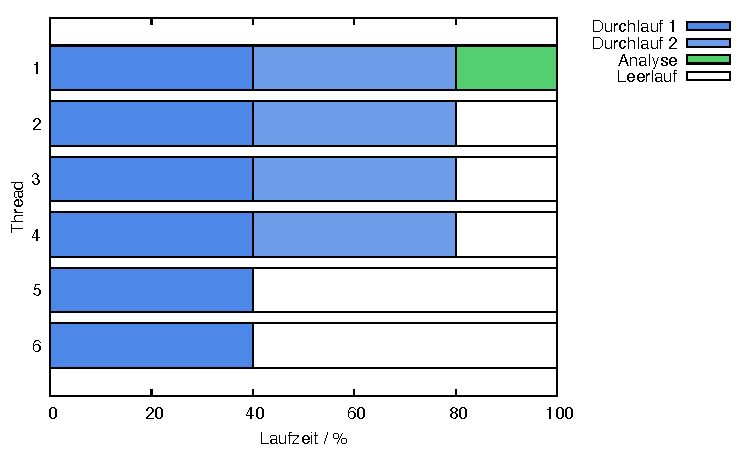
\includegraphics[width=0.8\textwidth]{../results/plots/timeline/timeline_plot_6threads.pdf}
  \caption{Verteilung der Aufgaben auf die verfügbaren Threads bei einem Programmablauf mit 6 Threads}
  \label{fig:runtime_timeline_6threads}
\end{figure}

\begin{figure}[H]
  \centering
  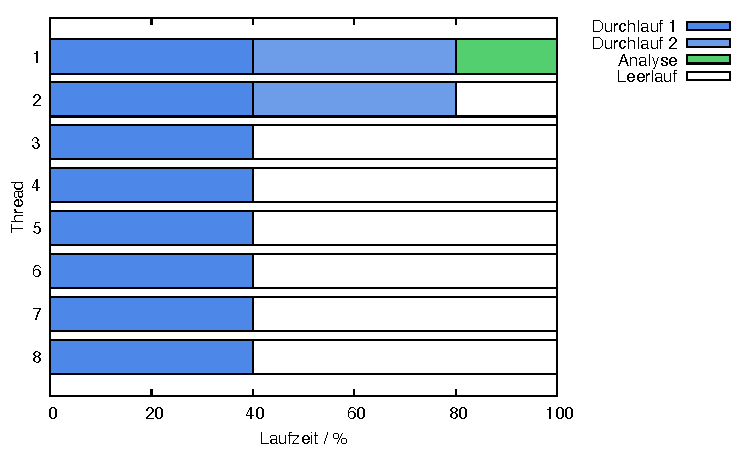
\includegraphics[width=0.8\textwidth]{../results/plots/timeline/timeline_plot_8threads.pdf}
  \caption{Verteilung der Aufgaben auf die verfügbaren Threads bei einem Programmablauf mit 8 Threads}
  \label{fig:runtime_timeline_8threads}
\end{figure}

Da für den Analyseschritt im Programmablauf alle 10 Ergebnisse benötigt werden, ist es algorithmisch nicht möglich, die Analyse vor Abschluss aller 10 Durchläufe auszuführen, um die Kerne, die im Leerlauf sind, zu nutzen. Es kann sich also nur eine gleichmäßige und effiziente Nutzung der Threads ergeben, wenn eine ganzzahlige Fraktion der gesamten Aufgaben als Threads zur Verfügung stehen. Bei 10 Aufgaben bedeutet das, dass 10, 5, 2 und 1 Thread ohne signifikanten Leerlauf der Threads voll ausgenutzt werden können, wenn man die Analyse auslässt.

Die Standardabweichung, welche in Tabelle \ref{tab:performance_comparison} zu sehen ist, ist insgesamt ziemlich gering, was für eine zuverlässige Verteilung der Threads von dem Betriebssystem  auf die verschiedenen Kerne spricht. Zu beobachten ist, dass die Standardabweichung selbstverständlich bei Tests, welche mehr Zeit beanspruchen höher ist, aber auch, dass bei diesem System die Standardabweichung bei 4 Threads verhältnismäßig leicht höher erscheint. Dies könnte eventuell an dem Scheduler des Kernels liegen, welcher dynamisch entscheidet, auf welchen Kernen Aufgaben laufen sollen.

\begin{figure}[H]
\centering
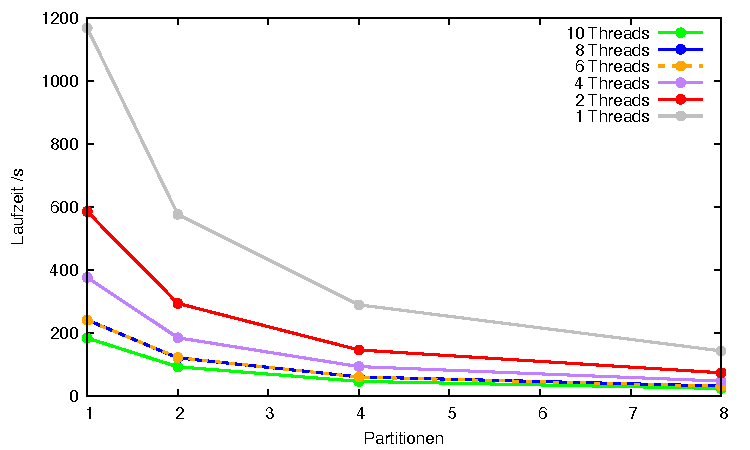
\includegraphics[width=0.8\textwidth]{../results/plots/3600xt/comp_all_threads.pdf}
\caption{Leistungstest auf AMD Ryzen 5 3600XT: Einfluss von Thread-Anzahlen auf Verarbeitungszeit bei variierenden Datensatzgrößen}
\label{fig:ryzen_benchmark_threads}
\end{figure}

\begin{figure}[H]
\centering
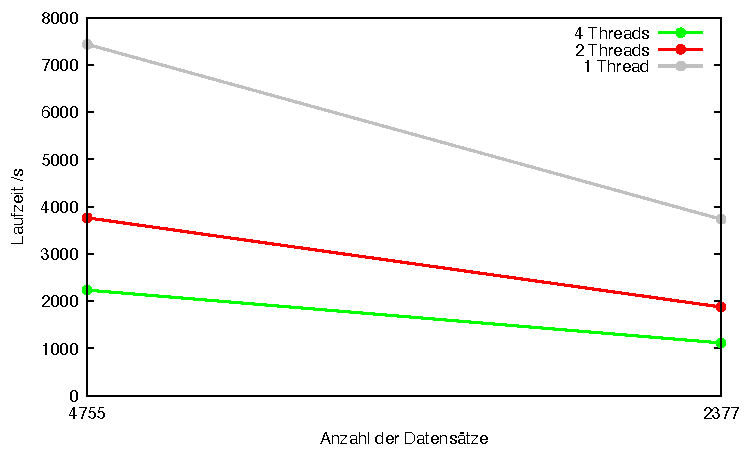
\includegraphics[width=0.8\textwidth]{../results/plots/raspberrypi3/comp_all_threads.pdf}
\caption{Leistungstest auf Raspberry Pi 3: Einfluss von Thread-Anzahlen auf Verarbeitungszeit bei variierenden Datensatzgrößen}
\label{fig:raspi_benchmark_threads}
\end{figure}

\begin{figure}[htbp!]
  \centering
  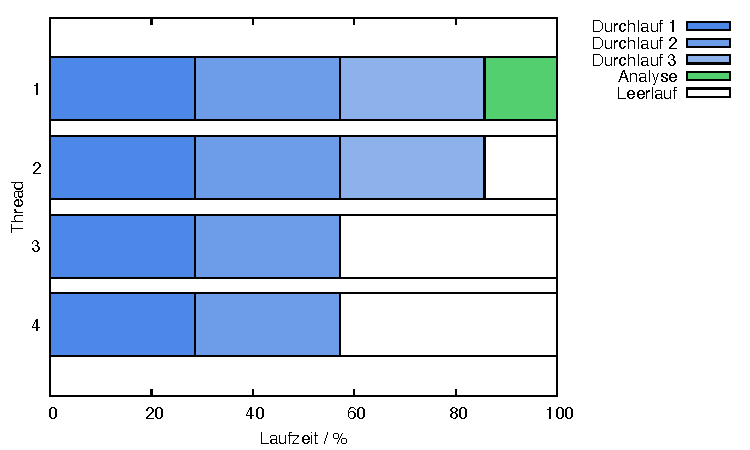
\includegraphics[width=0.8\textwidth]{../results/plots/timeline/timeline_plot_4threads.pdf}
  \caption{Verteilung der Aufgaben auf die verfügbaren Threads bei einem Programmablauf mit 8 Threads}
  \label{fig:runtime_timeline_4threads}
\end{figure}

\begin{figure}[H]
\centering
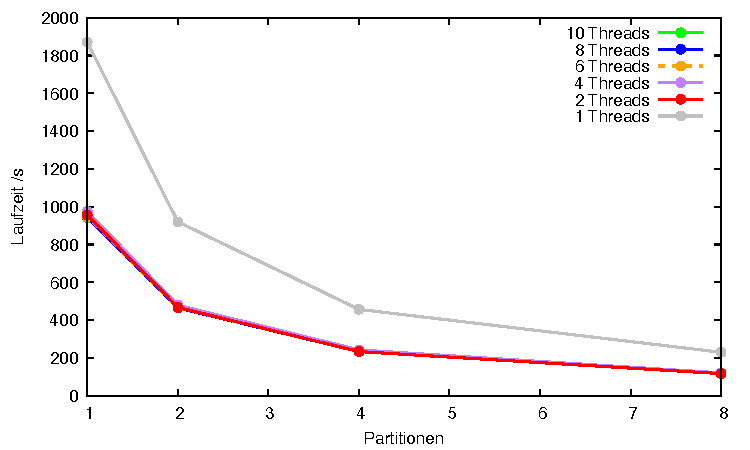
\includegraphics[width=0.8\textwidth]{../results/plots/vps/comp_all_threads.pdf}
\caption{Leistungstest auf AMD EPYC 7282 mit 2 verfügbaren Kernen: Einfluss von Thread-Anzahlen auf Verarbeitungszeit bei variierenden Datensatzgrößen}
\label{fig:vps_benchmark_threads}
\end{figure}

Des Weiteren ist der Overhead der Parallelisierung ein wichtiger Aspekt, der bei der Interpretation der Ergebnisse berücksichtigt werden muss. Trotz der Parallelisierung von Aufgaben bleibt der Overhead auf dem M1 Pro-Prozessor in diesem spezifischen Kontext gering, jedoch definitiv nicht vernachlässigbar. Die Skalierung der Leistung bleibt hoch. Für die gesamte Datensatzgröße von 19020 lag die benötigte Zeit bei einem Thread bei 948,6 Sekunden, während mit 10 Threads eine Zeit von 129,4 Sekunden erzielt wurde. Bei einer theoretisch perfekten Skalierung der Parallelisierung wären bei 10 Threads 94,86 Sekunden zu erwarten, jedoch läuft beispielsweise die Auswertung der Ergebnisse nach dem Programmablauf immer sequenziell, und benötigt somit gleich viel Zeit unabhängig von der verwendeten Thread Anzahl. Des Weiteren ist der bereits angesprochene Overhead der Parallelisierung ein Faktor. Dieser kann teilweise auf das Betriebssystem zurückzuführen sein, das Ressourcen für die Verwaltung und Koordination der Threads bereitstellen muss, was zu zusätzlicher Latenz führen kann, insbesondere wenn die CPU bereits stark ausgelastet ist. Bei voller CPU-Auslastung können Temperaturthrottling-Mechanismen eingreifen, um die Betriebstemperatur der CPU zu regulieren, was zu vorübergehenden Leistungseinbußen führen kann, da die Taktfrequenz reduziert wird, um die Temperaturen im sicheren Bereich zu halten. Ein weiterer Faktor ist die begrenzte Anzahl von Performance-Kernen auf dem M1 Pro Prozessor, die dazu führen kann, dass bei einer höheren Thread-Anzahl als verfügbaren Performance-Kernen nicht alle Threads auf gleich schnellen Kernen laufen können.

\mycomment{Beschriftung der Diagramme bei 1 Thread ist noch "1 Threads". Das sollte geändert werden.}

\section{Auswertung}

\begin{table}[H]
\centering
\caption{Benchmark-Ergebnisse für alle getesteten Systeme. Die benötigte Laufzeit $t$ ist ein Mittelwert aus jeweils mindestens 5 Durchläufen. Die Standardabweichung dieser Durchläufe ist mit $\sigma$ gekennzeichnet.}
\label{tab:performance_comparison}
\begin{adjustbox}{max width=\textwidth}
\renewcommand{\arraystretch}{1.5}
\begin{tabular}{ |c|r|S S|S S|S S|S S| } 
\hline & & \multicolumn{2}{c|}{M1 Pro} & \multicolumn{2}{c|}{Raspberry Pi} & \multicolumn{2}{c|}{\text{Ryzen 3600XT}} & \multicolumn{2}{c|}{VPS Server}\\
\text{Threads} & \text{Daten} & \text{Zeit} & \text{SD} & \text{Zeit} & \text{SD} & \text{Zeit}& \text{SD} & \text{Zeit} & \text{SD}  \\\hline
$1$ & $19020$ & 948,6 & 2,5 & \text{-} & \text{-} & 1167,2 & 4,3 & 1870,1 & 7,1 \\ 
$1$ & $9510$ & 478,8 & 9,7 & \text{-} & \text{-} & 575,6 & 8,3 & 919,9 & 1,5 \\ 
$1$ & $4755$ & 237,0 & 0,0 & 7436,2 & 19,6 & 288,5 & 1,0 & 456,7 & 1,3 \\ 
$1$ & $2377$ & 119,0 & 1,2 & 3734,3 & 36,3 & 142,2 & 2,2 & 229,6 & 0,9 \\ 
$2$ & $19020$ & 488,6 & 0,9 & \text{-} & \text{-} & 584,5 & 0,7 & 955,7 & 4,1 \\ 
$2$ & $9510$ & 244,4 & 0,5 & \text{-} & \text{-} & 292,9 & 0,0 & 466,9 & 2,7 \\ 
$2$ & $4755$ & 122,2 & 0,4 & 3764,5 & 33,9 & 145,1 & 0,3 & 233,3 & 1,8 \\ 
$2$ & $2377$ & 61,2 & 0,4 & 1876,1 & 12,0 & 72,6 & 0,2 & 116,6 & 0,7 \\ 
$4$ & $19020$ & 298,8 & 0,4 & \text{-} & \text{-} & 375,4 & 3,2 & 974,2 & 19,0 \\ 
$4$ & $9510$ & 149,6 & 0,5 & \text{-} & \text{-} & 183,9 & 7,3 & 478,6 & 3,1 \\ 
$4$ & $4755$ & 74,6 & 0,5 & 2235,2 & 6,1 & 92,3 & 2,4 & 242,0 & 2,1 \\ 
$4$ & $2377$ & 37,4 & 0,5 & 1117,0 & 2,0 & 46,2 & 1,4 & 120,3 & 1,2 \\ 
$6$ & $19020$ & 200,6 & 0,5 & \text{-} & \text{-} & 239,5 & 0,4 & 947,8 & 5,0 \\ 
$6$ & $9510$ & 100,2 & 0,4 & \text{-} & \text{-} & 121,0 & 0,3 & 465,8 & 2,6 \\ 
$6$ & $4755$ & 50,2 & 0,4 & \text{-} & \text{-} & 59,3 & 0,0 & 234,4 & 2,4 \\ 
$6$ & $2377$ & 25,2 & 0,4 & \text{-} & \text{-} & 29,7 & 0,1 & 117,5 & 1,6 \\ 
$8$ & $19020$ & 198,4 & 0,5 & \text{-} & \text{-} & 240,4 & 1,4 & 946,6 & 5,2 \\ 
$8$ & $9510$ & 99,4 & 0,5 & \text{-} & \text{-} & 120,1 & 0,5 & 464,3 & 1,8 \\ 
$8$ & $4755$ & 49,6 & 0,5 & \text{-} & \text{-} & 59,6 & 0,1 & 234,0 & 0,8 \\ 
$8$ & $2377$ & 24,8 & 0,4 & \text{-} & \text{-} & 30,4 & 1,3 & 116,8 & 0,8 \\ 
$10$ & $19020$ & 129,4 & 10,2 & \text{-} & \text{-} & 182,8 & 0,4 & 942,4 & 4,8 \\ 
$10$ & $9510$ & 60,6 & 3,6 & \text{-} & \text{-} & 91,7 & 0,9 & 466,6 & 1,3 \\ 
$10$ & $4755$ & 30,0 & 2,2 & \text{-} & \text{-} & 45,4 & 0,1 & 234,3 & 0,8 \\ 
$10$ & $2377$ & 14,6 & 0,5 & \text{-} & \text{-} & 22,8 & 0,1 & 117,1 & 0,6 \\ 
\hline \end{tabular} 

\end{adjustbox}
\end{table}
